% ============================================================
% Data and Methods — draft v2
% Citation keys resolve against references.bib (v. 2026-10-16d).
% Requires: natbib, booktabs, tabularx, tikz, amsmath, graphicx.
% Variant names are macros so that they can be renamed in one place.
%
% OPEN ITEMS FOR THIS SECTION (each is also marked TODO at its place):
%  [M1] PDOK: the study area was clipped manually. Add a bounds check to the analyzer,
%       record the clip bounds in the normalization manifest, then fill in the area
%       (Table tab:datasets-structure) and add PDOK to the study-area paragraph.
%  [M2] DONE: source and normalized statistics are generated from results.sqlite;
%       Table tab:datasets-normalized includes measured GPKG feature/vertex counts.
%       Raw PDOK GML vertex counts remain unavailable (not used in these tables).
%  [M3] Dataset provenance: data dates of BGT and NWI, swisstopo product name and nominal
%       scale; add one citation per dataset to the DATASETS section of references.bib.
%  [M4] Attributes: confirm that all attributes were kept for PDOK, USFWS, swisstopo and
%       OSM (only Natural Earth is reduced to a field subset in profile_rules.yaml).
%  [M5] DONE: Standard MVT samples for all maps are generated by manage.py maps;
%       zoom labels and explanatory text are typeset in LaTeX.
%  [M6] Check the qualitative dataset characterizations against tile-level statistics.
%  [M7] DONE: both formats are recompressed at gzip level 6, mtime=0 for analysis;
%       stored lengths are retained and compared in gzip_check.
%  [M8] DONE (from output_analysis_core.py): ratio of sums; deduplicated tiles counted
%       per address; headline gzip sizes use deterministic recompression.
%  [M9] Not for the paper: in the OSM profile, layer "buildings" holds all points,
%       lines, polygons and other relations, "transportation" holds route relations.
%       Describe OSM layers by content in Results; consider renaming in the profile.
%  [M10] Before publishing code: remove the inactive netherlands_amsterdam profile and the
%       copied PDOK prefixes in the OSM profile; move PeakMemory/get_output_size out of
%       the legacy .planetiler module imported by gdal_tiles.py.
% ============================================================

\providecommand{\VStd}{Standard}
\providecommand{\VDfour}{Dense-4}
\providecommand{\VDsixteen}{Dense-16}

\section{Data and Methods}
\label{sec:method}

The experiment converts five heterogeneous vector datasets into tile pyramids in five
variants, encodes every variant in MVT, MLT v1 and MLT v2, and compares the paired
encodings tile by tile. Preparation is
split into two stages: Stage~A normalizes each raw source once into a canonical
GeoPackage, and Stage~B generates all tile variants from that GeoPackage, so that the
variants of one dataset differ only in tiling parameters.

% ------------------------------------------------------------
\subsection{Datasets}
\label{sec:data}

The corpus was chosen to cover different ways in which geospatial data are produced,
because the production process largely determines how much geometry and how many
attributes a map carries per unit area. It contains a generalized small-scale reference
map (Natural Earth), a national large-scale topographic register (PDOK), two thematic
survey products (USFWS wetlands and the swisstopo geological map) and a crowdsourced
dataset (OpenStreetMap). Table~\ref{tab:datasets-provenance} lists their provenance and
Figure~\ref{fig:datasets} shows samples.

Processing whole national or global datasets at three granularities exceeded the memory
and time available for the GDAL-based pipeline, so each dataset was clipped to a study
area (Table~\ref{tab:datasets-structure}). The areas were chosen to contain dense content
for each dataset: the eastern United States for Natural Earth, the Säntis region of
north-eastern Switzerland for the swisstopo map, and the same $0.4^\circ\times0.4^\circ$
area around New Orleans for both USFWS and OSM. The last choice gives a matched pair: two
datasets with very different content over identical geography, which helps to separate
the effect of content from that of location.
% TODO [M1]: add the PDOK study area here once its clip bounds are recorded
%            (PDOK was clipped manually, outside the profile).


\begin{table*}[!tp]
\centering
\caption{Provenance and characteristics of the five datasets.}
\label{tab:datasets-provenance}
\small
\begin{tabularx}{\textwidth}{
    @{}l
    >{\raggedright\arraybackslash}p{3.0cm}
    >{\raggedright\arraybackslash}X
    >{\raggedright\arraybackslash}p{2.1cm}
    >{\raggedright\arraybackslash}p{2.1cm}
    @{}
}
\toprule
Dataset &
Producer &
Content and production mode &
Nominal scale &
Data date \\
\midrule

Natural Earth &
NACIS &
Global physical and cultural reference layers;
generalized cartography at three scales &
1:10m--1:110m &
2021-12 \\

\addlinespace

PDOK BGT &
Dutch public authorities via PDOK &
Large-scale topographic base register
(buildings, roads, land cover, street furniture);
authoritative, continuously updated data &
1:500--1:5{,}000 &
2026-07
(snapshot, approx.) \\

\addlinespace

USFWS wetlands &
U.S.\ Fish and Wildlife Service (NWI) &
Wetland and deepwater habitat polygons for
Louisiana; Cowardin classification;
photo-interpreted thematic mapping &
1:24{,}000 &
2026-05
(release) \\

\addlinespace

swisstopo geology &
Federal Office of Topography swisstopo &
Structural Map of the Helvetic Zone,
Geological Special Map No.~128;
stratigraphic units, folds and tectonic
structures; compiled geological mapping &
1:100{,}000 &
2011
(vector edition) \\

\addlinespace

OSM Louisiana &
OpenStreetMap contributors &
Buildings, transport, land use and points
of interest for Louisiana;
crowdsourced geographic data &
Variable &
2026-09-12 \\

\bottomrule
\end{tabularx}

\vspace{2pt}
\begin{minipage}{\textwidth}
\footnotesize
\textit{Note.}
Dates refer to the dataset version or acquisition snapshot
used in the experiments, not necessarily to the dates of
original field surveys or imagery.
PDOK BGT is continuously updated; its snapshot month
is approximate.
The USFWS date denotes the May 2026 NWI release.
The swisstopo date denotes the 2011 vector edition
of Geological Special Map No.~128 (original map: 2010).
Map scales describe source cartography rather than
the zoom levels of the generated vector tiles.
\end{minipage}
\end{table*}

\begin{table*}[!tp]
\centering
\caption{Raw sources and study areas. Size, source layers, features and fields refer
to the whole raw source; fields are distinct attribute columns summed over layers (for
OSM, tag keys exposed by the GDAL OSM driver). Tile layers and the logical zoom range
refer to the tiled study area. Areas are geodesic areas of declared clipping bounds;
an em dash denotes missing bounds (PDOK). Small extent overruns for USFWS and
swisstopo are recorded in the analysis checks.}
\label{tab:datasets-structure}
\small
\setlength{\tabcolsep}{4pt}
\begin{tabular}{@{}l r r r r r r c@{}}
\toprule
 & \multicolumn{4}{c}{Raw source} & \multicolumn{3}{c}{Study area} \\
\cmidrule(lr){2-5}\cmidrule(l){6-8}
Dataset & MB & Layers & Features & Fields & km$^2$ & Tile layers & Zoom \\
\midrule
% Generated by analysis.extended_report from hash-verified inventories and extended tiles.
Natural Earth & 446 & 183 & 350{,}371 & 12{,}762 & 4.4\,M & 5 & 4--11 \\
PDOK BGT & 53 & 26 & 190{,}294 & 379 & --- & 10 & 3--14 \\
USFWS & 1{,}328 & 4 & 657{,}058 & 21 & 1{,}719 & 1 & 3--14 \\
swisstopo & 46 & 4 & 16{,}319 & 47 & 737 & 1 & 3--14 \\
OSM & 146 & 5 & 1{,}863{,}746 & 3{,}300 & 1{,}719 & 2 & 4--14 \\
\bottomrule

\end{tabular}
% Data rows: analysis.paper_tables, results.sqlite. TODO [M1]: PDOK bounds.
\end{table*}

\begin{table*}[!tp]
\centering
\caption{Measured structure of the normalized GeoPackages used for tile generation.
Size is the on-disk GeoPackage size in MiB; features, vertices and attribute fields
are summed over its layers.}
\label{tab:datasets-normalized}
\small
\begin{tabular}{@{}l r r r r r@{}}
\toprule
Dataset & MiB & Layers & Features & Vertices & Fields \\
\midrule
% Generated by analysis.extended_report from hash-verified inventories and extended tiles.
Natural Earth & 86.5 & 183 & 60{,}574 & 3{,}401{,}476 & 11{,}048 \\
PDOK BGT & 222.3 & 26 & 190{,}294 & 8{,}915{,}989 & 379 \\
USFWS & 108.6 & 4 & 41{,}781 & 5{,}840{,}438 & 21 \\
swisstopo & 0.8 & 1 & 213 & 34{,}560 & 10 \\
OSM & 14.9 & 5 & 15{,}621 & 722{,}903 & 584 \\
\bottomrule

\end{tabular}
\end{table*}

The datasets differ along the dimensions that matter for a columnar encoder.
Natural Earth has few features per unit area but many layers and attributes.
USFWS consists almost entirely of one polygon layer with very detailed boundaries,
about 210 vertices per feature in the raw source, and few attributes. PDOK is dense in
features of many classes with rich attribute schemas. The swisstopo map has few features
over a small area. OSM combines dense buildings with sparser lines and points and a very
large, sparse tag vocabulary.
% TODO [M6]: check these characterizations against tile-level statistics.

Figure~\ref{fig:datasets} shows three nested views per dataset from the \VStd{}
MVT archives. The stored zoom levels and tile addresses were selected for each map's
characteristic content and fixed in a reproducible region configuration. Square
viewports lie inside both the selected tile and the dataset bounds at that zoom;
clipped margins outside those bounds are excluded. Magenta outlines mark the next
view, while zoom labels and palette explanations are typeset in LaTeX. OSM and USFWS
use the same viewports for a direct comparison of coastal Louisiana. Complete tile
addresses, viewport bounds, approximate ground sizes and color inventories are
exported with the figures.

% Generated by python manage.py maps; text stays in LaTeX.
\begin{figure*}[p]
\centering
\begingroup
\setlength{\tabcolsep}{2pt}
\renewcommand{\arraystretch}{1}
\begin{tabular}{@{}cccc@{}}
\begin{minipage}[t]{0.205\textwidth}\vspace{0pt}\centering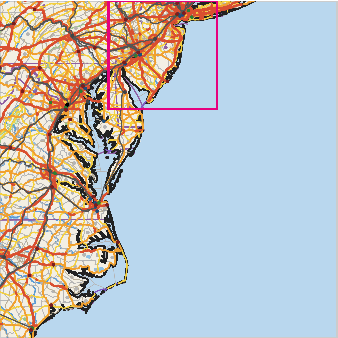
\includegraphics[width=\linewidth]{figures/map_natural_earth_vector_z5.pdf}\par\vspace{1pt}\scriptsize $z=5$\end{minipage} & \begin{minipage}[t]{0.205\textwidth}\vspace{0pt}\centering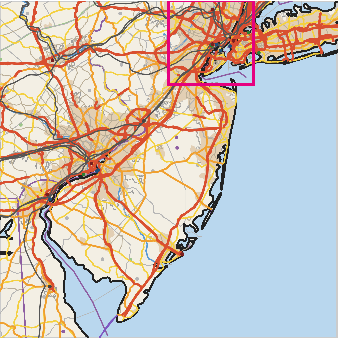
\includegraphics[width=\linewidth]{figures/map_natural_earth_vector_z7.pdf}\par\vspace{1pt}\scriptsize $z=7$\end{minipage} & \begin{minipage}[t]{0.205\textwidth}\vspace{0pt}\centering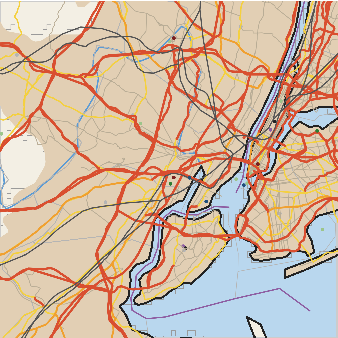
\includegraphics[width=\linewidth]{figures/map_natural_earth_vector_z9.pdf}\par\vspace{1pt}\scriptsize $z=9$\end{minipage} & \begin{minipage}[t]{0.34\textwidth}\vspace{1pt}\footnotesize\raggedright \textbf{(a) Natural Earth}\\ New York / New Jersey.\par\smallskip Colors are illustrative: blue water, pale land, tan urban areas, green parks, red/orange/yellow roads, purple state boundaries and gray county boundaries. Points mark places and transport facilities. Source: Natural Earth / NACIS.\end{minipage} \\[5pt]
\begin{minipage}[t]{0.205\textwidth}\vspace{0pt}\centering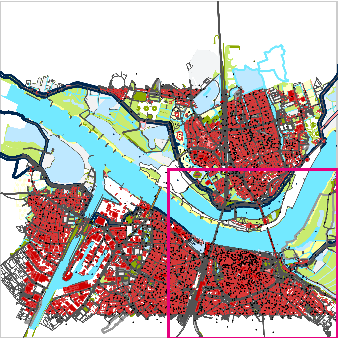
\includegraphics[width=\linewidth]{figures/map_pdok_netherlands_infrostructure_z12.pdf}\par\vspace{1pt}\scriptsize $z=12$\end{minipage} & \begin{minipage}[t]{0.205\textwidth}\vspace{0pt}\centering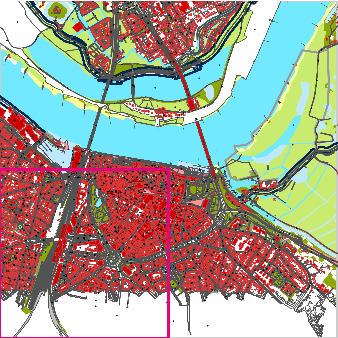
\includegraphics[width=\linewidth]{figures/map_pdok_netherlands_infrostructure_z13.pdf}\par\vspace{1pt}\scriptsize $z=13$\end{minipage} & \begin{minipage}[t]{0.205\textwidth}\vspace{0pt}\centering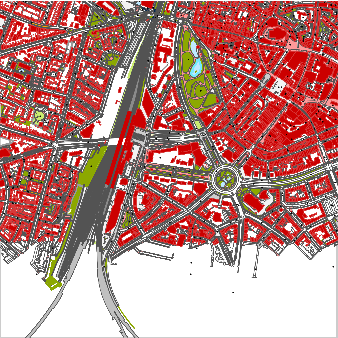
\includegraphics[width=\linewidth]{figures/map_pdok_netherlands_infrostructure_z14.pdf}\par\vspace{1pt}\scriptsize $z=14$\end{minipage} & \begin{minipage}[t]{0.34\textwidth}\vspace{1pt}\footnotesize\raggedright \textbf{(b) PDOK BGT}\\ Nijmegen, Netherlands.\par\smallskip The palette follows the BGT standard visualization: red buildings, blue water, green vegetation and white local roads/paved areas; gray denotes classes without an assigned standard color. Source: PDOK.\end{minipage} \\[5pt]
\begin{minipage}[t]{0.205\textwidth}\vspace{0pt}\centering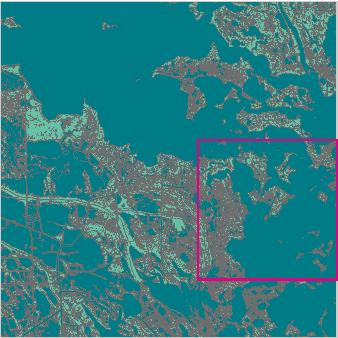
\includegraphics[width=\linewidth]{figures/map_usfws_luisiana_wetlands_geopackage_z10.pdf}\par\vspace{1pt}\scriptsize $z=10$\end{minipage} & \begin{minipage}[t]{0.205\textwidth}\vspace{0pt}\centering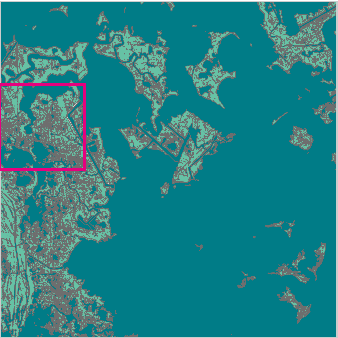
\includegraphics[width=\linewidth]{figures/map_usfws_luisiana_wetlands_geopackage_z12.pdf}\par\vspace{1pt}\scriptsize $z=12$\end{minipage} & \begin{minipage}[t]{0.205\textwidth}\vspace{0pt}\centering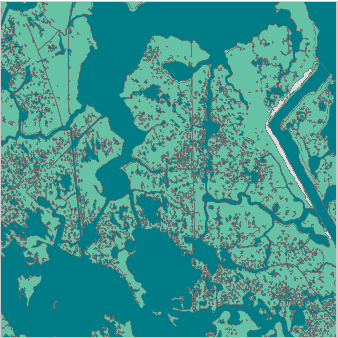
\includegraphics[width=\linewidth]{figures/map_usfws_luisiana_wetlands_geopackage_z14.pdf}\par\vspace{1pt}\scriptsize $z=14$\end{minipage} & \begin{minipage}[t]{0.34\textwidth}\vspace{1pt}\footnotesize\raggedright \textbf{(c) USFWS wetlands}\\ coastal Louisiana.\par\smallskip The NWI palette distinguishes forested/shrub wetlands (dark green), emergent wetlands (light green), tidal wetlands (teal), and water classes (blue); unclassified polygons are light gray. Source: U.S. Fish and Wildlife Service, National Wetlands Inventory.\end{minipage} \\[5pt]
\begin{minipage}[t]{0.205\textwidth}\vspace{0pt}\centering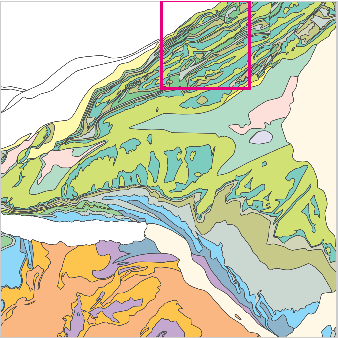
\includegraphics[width=\linewidth]{figures/map_swisstopo_mountains_vector_z10.pdf}\par\vspace{1pt}\scriptsize $z=10$\end{minipage} & \begin{minipage}[t]{0.205\textwidth}\vspace{0pt}\centering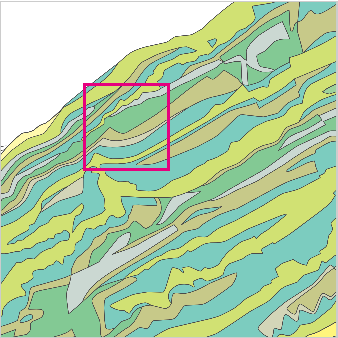
\includegraphics[width=\linewidth]{figures/map_swisstopo_mountains_vector_z12.pdf}\par\vspace{1pt}\scriptsize $z=12$\end{minipage} & \begin{minipage}[t]{0.205\textwidth}\vspace{0pt}\centering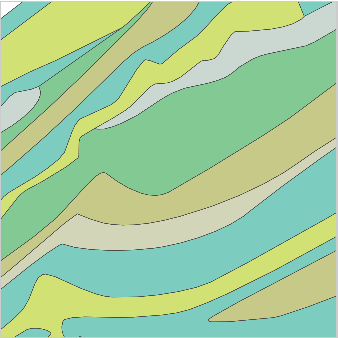
\includegraphics[width=\linewidth]{figures/map_swisstopo_mountains_vector_z14.pdf}\par\vspace{1pt}\scriptsize $z=14$\end{minipage} & \begin{minipage}[t]{0.34\textwidth}\vspace{1pt}\footnotesize\raggedright \textbf{(d) swisstopo geology}\\ Saentis, Switzerland.\par\smallskip Colors distinguish geological units using the swisstopo legend and the retained \texttt{SYMBOL}/\texttt{INDEX\_} attributes. White denotes units without an assigned legend color. Source: swisstopo, Structural Map of the Helvetic Zone, sheet 128.\end{minipage} \\[5pt]
\begin{minipage}[t]{0.205\textwidth}\vspace{0pt}\centering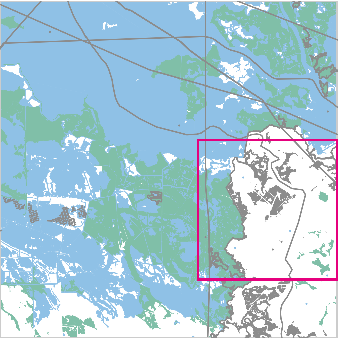
\includegraphics[width=\linewidth]{figures/map_louisiana-260912_z10.pdf}\par\vspace{1pt}\scriptsize $z=10$\end{minipage} & \begin{minipage}[t]{0.205\textwidth}\vspace{0pt}\centering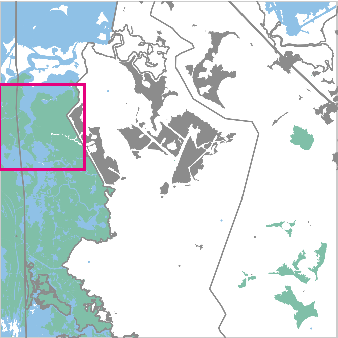
\includegraphics[width=\linewidth]{figures/map_louisiana-260912_z12.pdf}\par\vspace{1pt}\scriptsize $z=12$\end{minipage} & \begin{minipage}[t]{0.205\textwidth}\vspace{0pt}\centering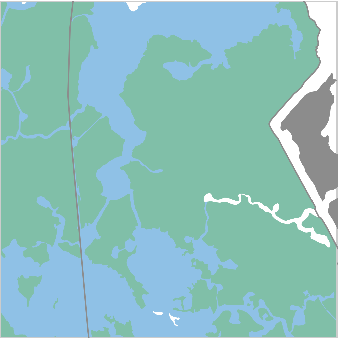
\includegraphics[width=\linewidth]{figures/map_louisiana-260912_z14.pdf}\par\vspace{1pt}\scriptsize $z=14$\end{minipage} & \begin{minipage}[t]{0.34\textwidth}\vspace{1pt}\footnotesize\raggedright \textbf{(e) OpenStreetMap}\\ coastal Louisiana.\par\smallskip An illustrative tag-based palette shows water in blue, wetlands in teal, vegetation in green, buildings in brown, roads/routes in orange and other objects in gray. Classification uses retained OSM tags rather than merged tile-layer names. Source: \copyright{} OpenStreetMap contributors, ODbL.\end{minipage} \\[5pt]
\end{tabular}
\endgroup
\caption{The five datasets at three zoom levels, rendered from Standard MVT tiles. Views are nested from left to right; magenta outlines locate the next view. Square viewports stay within the configured data bounds at each zoom. USFWS and OSM show the same coastal Louisiana areas.}
\label{fig:datasets}
\label{fig:map-natural_earth_vector}
\label{fig:map-pdok_netherlands_infrostructure}
\label{fig:map-usfws_luisiana_wetlands_geopackage}
\label{fig:map-swisstopo_mountains_vector}
\label{fig:map-louisiana-260912}
\end{figure*}



% ------------------------------------------------------------
\subsection{Normalization}
\label{sec:normalization}

Each raw source was converted with GDAL into a canonical GeoPackage in Web Mercator
(EPSG:3857) with two-dimensional geometries, clipped once to the study area and indexed
spatially. Source layers were mapped onto a common set of semantic kinds (water, land,
boundary, transport, place, building, infrastructure, terrain) so that all datasets can
be rendered with one style sheet and inspected visually. Several source layers can be
merged into one tile layer, which gives between one (USFWS) and ten (PDOK) tile layers per
dataset (Table~\ref{tab:datasets-structure}). For Natural Earth, which has 183 source
layers with heterogeneous schemas, only a common subset of attributes (feature class,
names in four languages, administrative codes and rank fields) was kept. Geometry is not
altered by this mapping.
% TODO [M4]: confirm that all attributes were kept for the other four datasets.
% NOTE [M9]: OSM layer names do not match their content (see header).
A manifest records the source and rule hashes, CRS, bounds, layer counts, feature
identity strategy and GDAL version, so that every normalized layer can be traced back to
its source.

The grouping of source layers into tile layers affects the absolute size of both
encodings, and of MLT in particular, because it determines how many features share one
set of streams. The mapping rules are identical for all variants of a dataset and for
both encodings. However, changing tile granularity can change which property types
co-occur within an output layer, so the resulting type conversions are measured
separately (Section~\ref{sec:encoding}).

% ------------------------------------------------------------

\subsection{Tile generation and source identity}\label{sec:tile-generation}
MVT is regenerated with GDAL 3.13.3 from the same normalized sources and study
regions. Globally unique feature IDs equal original GeoPackage FIDs plus disjoint
source-layer offsets. A separate SQLite table maps these IDs to original layers and
FIDs. A derived GeoPackage materializes only this FID remapping; exhaustive SQL
comparison verifies that every geometry BLOB and attribute cell equals the source.
GDAL's \texttt{-preserve\_fid} writes the IDs into MVT; no provenance attribute is
added. IDs identify normalized records, including distinct records in different layers
that describe the same real-world object. Historical archives are stored separately.

Standard and Dense retain the original layer grouping and generation rules:
simplification is 1.6 tile units below the maximum zoom and 1.0 at maximum zoom;
buffer width is 80 units per 4096 extent units. Extent scales with linear cell width,
preserving the intended ground-coordinate resolution at matched logical zoom.
Tile-size and feature limits are $2^{31}-1$. GDAL writes MBTiles and directly repacks
MVT payloads into PMTiles~\citep{gdal_mvt,pmtiles_v3}.

\subsection{Five variants and three comparisons}\label{sec:granularity}
Standard uses extent 4096. Aggregated-4 and Aggregated-16 regroup $2\times2$ and
$4\times4$ Standard cells into one unit, translating coordinates by integer multiples
of 4096. They retain the exact feature multiset: geometry command sequences, precision,
fragments, duplicates, ID presence, attributes and typed protobuf values. MVT keys and
values are interned across children, giving MVT the enlarged dictionary scope too.
No feature is merged, deduplicated, simplified or regenerated. An independent parse
of every serialized aggregate must reproduce the translated typed multiset.
Dense instead regenerates the larger cell, changing clipping, buffering and possibly
representation. Figure~\ref{fig:variants} illustrates the Dense spatial arrangement;
Aggregated uses the same parent layout while retaining internal Standard fragments.

\begin{table}[!tbp]\centering\small
\caption{Five variants. Offset $d$ relates stored zoom $z$ to logical zoom
$\ell=z+d$. Factor denotes geographic area relative to a Standard cell.}
\label{tab:variants}\setlength{\tabcolsep}{3pt}
\begin{tabular}{@{}lrrrl@{}}\toprule
Variant & Factor & Extent & $d$ & Content\\
\midrule% Generated by analysis.extended_report from measured extended results; do not edit.
Standard & 1 & 4096 & 0 & Conventional baseline \\
Aggregated-4 & 4 & 8192 & 1 & Exact Standard multiset \\
Aggregated-16 & 16 & 16384 & 2 & Exact Standard multiset \\
Dense-4 & 4 & 8192 & 1 & Regenerated \\
Dense-16 & 16 & 16384 & 2 & Regenerated \\
\bottomrule
\end{tabular}\end{table}
% Figure: Standard pyramid vs. Dense-4 / Dense-16 stored tiles.
% Requires: \usepackage{tikz}; variant-name macros \VStd, \VDfour, \VDsixteen.
\begin{figure}[t]
\centering
\begin{tikzpicture}[x=1cm, y=1cm, font=\scriptsize,
    unit/.style={draw=black!70, fill=black!8},
    dense/.style={draw=black, very thick, fill=black!22},
    lab/.style={align=center, text width=2.5cm, anchor=north}]
  \def\S{1.8}
  % ---- (a) Standard pyramid: separately encoded tiles ----
  \node[anchor=west, font=\footnotesize\bfseries] at (-0.1,2.55)
    {(a) \VStd{} pyramid: every tile encoded separately};
  \foreach \n/\x/\lbl in {1/0/{zoom $z$\\1 tile}, 2/2.6/{zoom $z{+}1$\\4 tiles}, 4/5.2/{zoom $z{+}2$\\16 tiles}} {
    \pgfmathsetmacro{\c}{\S/\n}
    \foreach \i in {1,...,\n} \foreach \j in {1,...,\n}
      \draw[unit] ({\x+(\i-1)*\c},{(\j-1)*\c+0.25}) rectangle ++(\c,\c);
    \node[lab] at (\x+\S/2,0.2) {\lbl};
  }
  % ---- (b) stored tile at z/x/y ----
  \node[anchor=west, font=\footnotesize\bfseries] at (-0.1,-1.25)
    {(b) One stored tile at address $z/x/y$};
  \draw[unit] (0,-3.4) rectangle ++(\S,\S);
  \node[lab] at (\S/2,-3.45) {\VStd\\content of $z$\\extent 4096};
  \draw[dense] (2.6,-3.4) rectangle ++(\S,\S);
  \draw[dashed, black!60] (2.6+\S/2,-3.4) -- ++(0,\S) (2.6,-3.4+\S/2) -- ++(\S,0);
  \node[lab] at (2.6+\S/2,-3.45) {\VDfour\\content of $z{+}1$\\extent 8192};
  \draw[dense] (5.2,-3.4) rectangle ++(\S,\S);
  \foreach \k in {1,2,3} {
    \draw[dashed, black!60] (5.2+\k*\S/4,-3.4) -- ++(0,\S);
    \draw[dashed, black!60] (5.2,-3.4+\k*\S/4) -- ++(\S,0);
  }
  \node[lab] at (5.2+\S/2,-3.45) {\VDsixteen\\content of $z{+}2$\\extent 16384};
  % arrows from (a) to (b)
  \foreach \x in {0,2.6,5.2}
    \draw[-{Stealth}, black!60] (\x+\S/2,-0.55) -- (\x+\S/2,-1.05);
\end{tikzpicture}
\caption{Spatial-granularity variants. (a)~In the \VStd{} pyramid an area at
logical zoom $z+1$ or $z+2$ is partitioned into 4 or 16 independently encoded tiles.
(b)~The \VDfour{} and \VDsixteen{} variants generate one independently encoded tile
over the corresponding parent area using the feature-selection and simplification rules
of logical zoom $z+1$ or $z+2$. Coordinate extent grows with the linear spatial factor
to preserve approximately the same ground-coordinate precision; extent is not itself
the granularity variable. Aggregated-4 and Aggregated-16 use these same larger
footprints and extents, but translate and retain the complete Standard feature
multiset instead of regenerating it. Dashed lines mark the internal Standard
boundaries; their existing fragments and buffered copies remain in Aggregated.}
\label{fig:variants}
\end{figure}


At each logical zoom, comparisons match parent-cell coordinates over the geographic
intersection of available Standard groups, Aggregated and Dense blocks. Missing
edge blocks are reported separately. Standard--Aggregated measures the
\emph{compression-unit effect}; Aggregated--Dense measures the
\emph{tile-regeneration effect}; Standard--Dense measures the total effect.
The regeneration effect is not attributed exclusively to clipping.

\subsection{Pinned Rust encoding and validation}\label{sec:encoding}
Both versions use the official \texttt{mlt-core 0.22.1} source shipped with
\texttt{maplibre-tiles 0.4.1}~\citep{maplibre_tiles_py,maplibre_mlt_rust_pinned}.
A framed CLI adapter calls Rust directly; Python handles archive I/O. Source SHA-256,
Cargo lockfile, Rust version, binary and adapter hashes, and settings accompany each
conversion. Both versions use Native/4G with tessellation and sorting disabled,
FSST, FastPFOR and shared dictionaries enabled. Fixed v2 defaults enable packed
dictionary codes and disable ALP, float dictionaries, second-order delta and rANS
vertices. We do not search codec options.

Every encoded layer is decoded and compared to the Rust MVT importer's layer using
the official CLI verification rules. Those rules permit integer-width changes,
polygon winding normalization and absent/null equivalence. The importer can unify
mixed property types, including string coercion; per-property source types and
imported column types are exported. Thus the round trip checks consistency after
import, not strict equality to every typed MVT value. Source/imported feature and
vertex counts expose additional normalization. Aggregation uses its own stronger
typed-protobuf multiset check before MLT encoding.
Exact equivalence is established at the MVT input boundary. Since column-type
unification depends on the values sharing a unit, Aggregated MLT can normalize
types differently from Standard MLT. The measured fixed-input byte effect includes
this format constraint; it does not isolate compression mechanics from normalization.

Earlier historical validation failed at 48 addresses under an internal 20 MiB Rust
guard: 22 Natural Earth, 25 PDOK and one USFWS. The stock 64 MiB guard in 0.4.1
still rejected 17 of those addresses. The extended CLI passes 256 MiB explicitly
to MVT import, MLT parsing, decoding and the read-only structural walker. This guard
is distinct from Docker's quota and does not bound total RSS. The largest new
PDOK Dense-16 input exposed a separate 32 MiB protobuf element-memory guard;
raising only the MLT decoder budget did not affect that earlier import stage.
Budget-only patches expose explicit limits through both readers and the walker;
their original defaults and encoding algorithms remain unchanged.
After writing, every physical PMTiles archive is read back. Its addresses, raw
lengths and payload hashes must match the measurements, linking native validation
to the actual stored MLT bytes and detecting missing or changed payloads.

\subsection{Measurements and additive decomposition}\label{sec:metrics}
Raw bytes and independently recompressed gzip bytes (level 6, timestamp zero) are
measured per address. Unique stored payloads and complete archive sizes are recorded
separately. MLT saving within one variant is
\begin{equation}\label{eq:saving}
S=100\left(1-\frac{\sum B_{\rm MLT}}{\sum B_{\rm MVT}}\right).
\end{equation}
For one format and compression state over identical matched blocks, let $B_S$,
$B_A$ and $B_D$ denote Standard, Aggregated and Dense bytes. Then
\begin{equation}\label{eq:decomposition}
\underbrace{B_S-B_D}_{\text{total}}=
\underbrace{B_S-B_A}_{\text{aggregation}}+
\underbrace{B_A-B_D}_{\text{regeneration}}.
\end{equation}
Component percentages all divide by $B_S$ and remain additive. They are distinct
from MLT-versus-MVT percentage-point gains.

Content counts include feature instances, unique provenance IDs at each logical
zoom, explicit stored vertices and MoveTo components. Components include line parts,
rings and points; they are not necessarily clipping fragments. Repeated instances
share an ID. Repeated vertices share ID and integer coordinates within a comparison
block; implicit polygon closures are excluded. These are observable redundancy
measures, not a causal partition into clipping and buffering. Identities are not
deduplicated across logical zooms.

The official version-aware annotated walker partitions each MLT frame into metadata
and encoded data regions. For frame bytes $F$ and stream payload bytes $P$,
\begin{equation}\label{eq:structural-share}R_{\rm struct}=(F-P)/F.\end{equation}
Stream length counts expanded logical values after integer RLE in both versions;
vertices count coordinate pairs, booleans logical positions. Values/stream and
payload bytes/value mix different stream roles. Structural statistics count each
unique MVT payload input once, while transfer sizes count addresses; they do not
provide an exact algebraic attribution of transfer savings to particular codecs.
